% 中期考核进展报告 — zjuthesis 兼容章节格式
% 编译：xelatex mid_term_report.tex
% 集成到 zjuthesis 时：将 \section 改为 \chapter，\subsection 改为 \section，依此类推

\documentclass[a4paper,12pt]{ctexart}
\usepackage{amsmath,amssymb}
\usepackage{tabularx}
\usepackage{booktabs}
\usepackage{graphicx}
\usepackage{geometry}
\usepackage{float}
\geometry{left=2.5cm,right=2.5cm,top=2.5cm,bottom=2.5cm}
\usepackage{hyperref}
\hypersetup{colorlinks=true,linkcolor=blue,citecolor=blue}

% 关闭 ctexart 自动编号，避免与手动中文编号冲突
\setcounter{secnumdepth}{0}

\graphicspath{{figures/}}

\title{\textbf{博士学位论文中期考核进展报告}\\[1em]
\large 深亚周期超快光脉冲的产生、探索及应用}
\author{党红亮\\指导教师：童利民 教授、 郭欣 教授\\光电科学与工程学院}
\date{}

\begin{document}
\maketitle

%==========================================================================
% 中期考核进展报告正文
%==========================================================================

围绕"深亚周期超快光脉冲的产生、探索及应用"这一课题，本文从理论方案的提出、量子力学基础框架的建立、纳米线高功率导波实验验证三个层面展开研究。截至目前，已发表 SCI 论文 1 篇，投稿 1 篇，另有 2 篇论文正在撰写中，实验平台建设按计划推进。以下分四个方面汇报进展。

%--------------------------------------------------------------------------
\section{一、已完成的任务及取得的成果}
%--------------------------------------------------------------------------

%------------------------------------------------------------------------------
\subsection{1.1 深亚周期超快光脉冲的理论预言（已发表）}
%------------------------------------------------------------------------------

将光脉冲压缩到半个光学周期以内，是超快光学领域一个长期未解决的基本问题。现有的阿秒脉冲技术（高次谐波产生）和光学参量放大技术所产生的脉冲，虽已短至数十阿秒，但本质上仍包含多个光学周期的载波振荡。当脉冲持续缩短到不足半个周期时，载波频率的概念不再成立，传统的振幅调制和相位锁定方法随之失效。

本文提出了一条全新的物理路径：利用纳米结构产生的深亚波长约束光场，与相对论性电子束发生逆康普顿散射（Inverse Compton Scattering, ICS），将空间维度的亚波长约束转化为时间维度的亚周期约束。图~\ref{fig:scheme} 展示了这一方案的基本思路——相对论电子与亚波长约束光场发生逆康普顿散射后，辐射脉冲的空间尺度被大幅压缩，从约半个波长（$\text{FWHM} \approx \lambda/2$）缩短至远小于半个波长（$\text{FWHM} \ll \lambda/2$），从而打破半周期极限。

\begin{figure}[H]
    \centering
    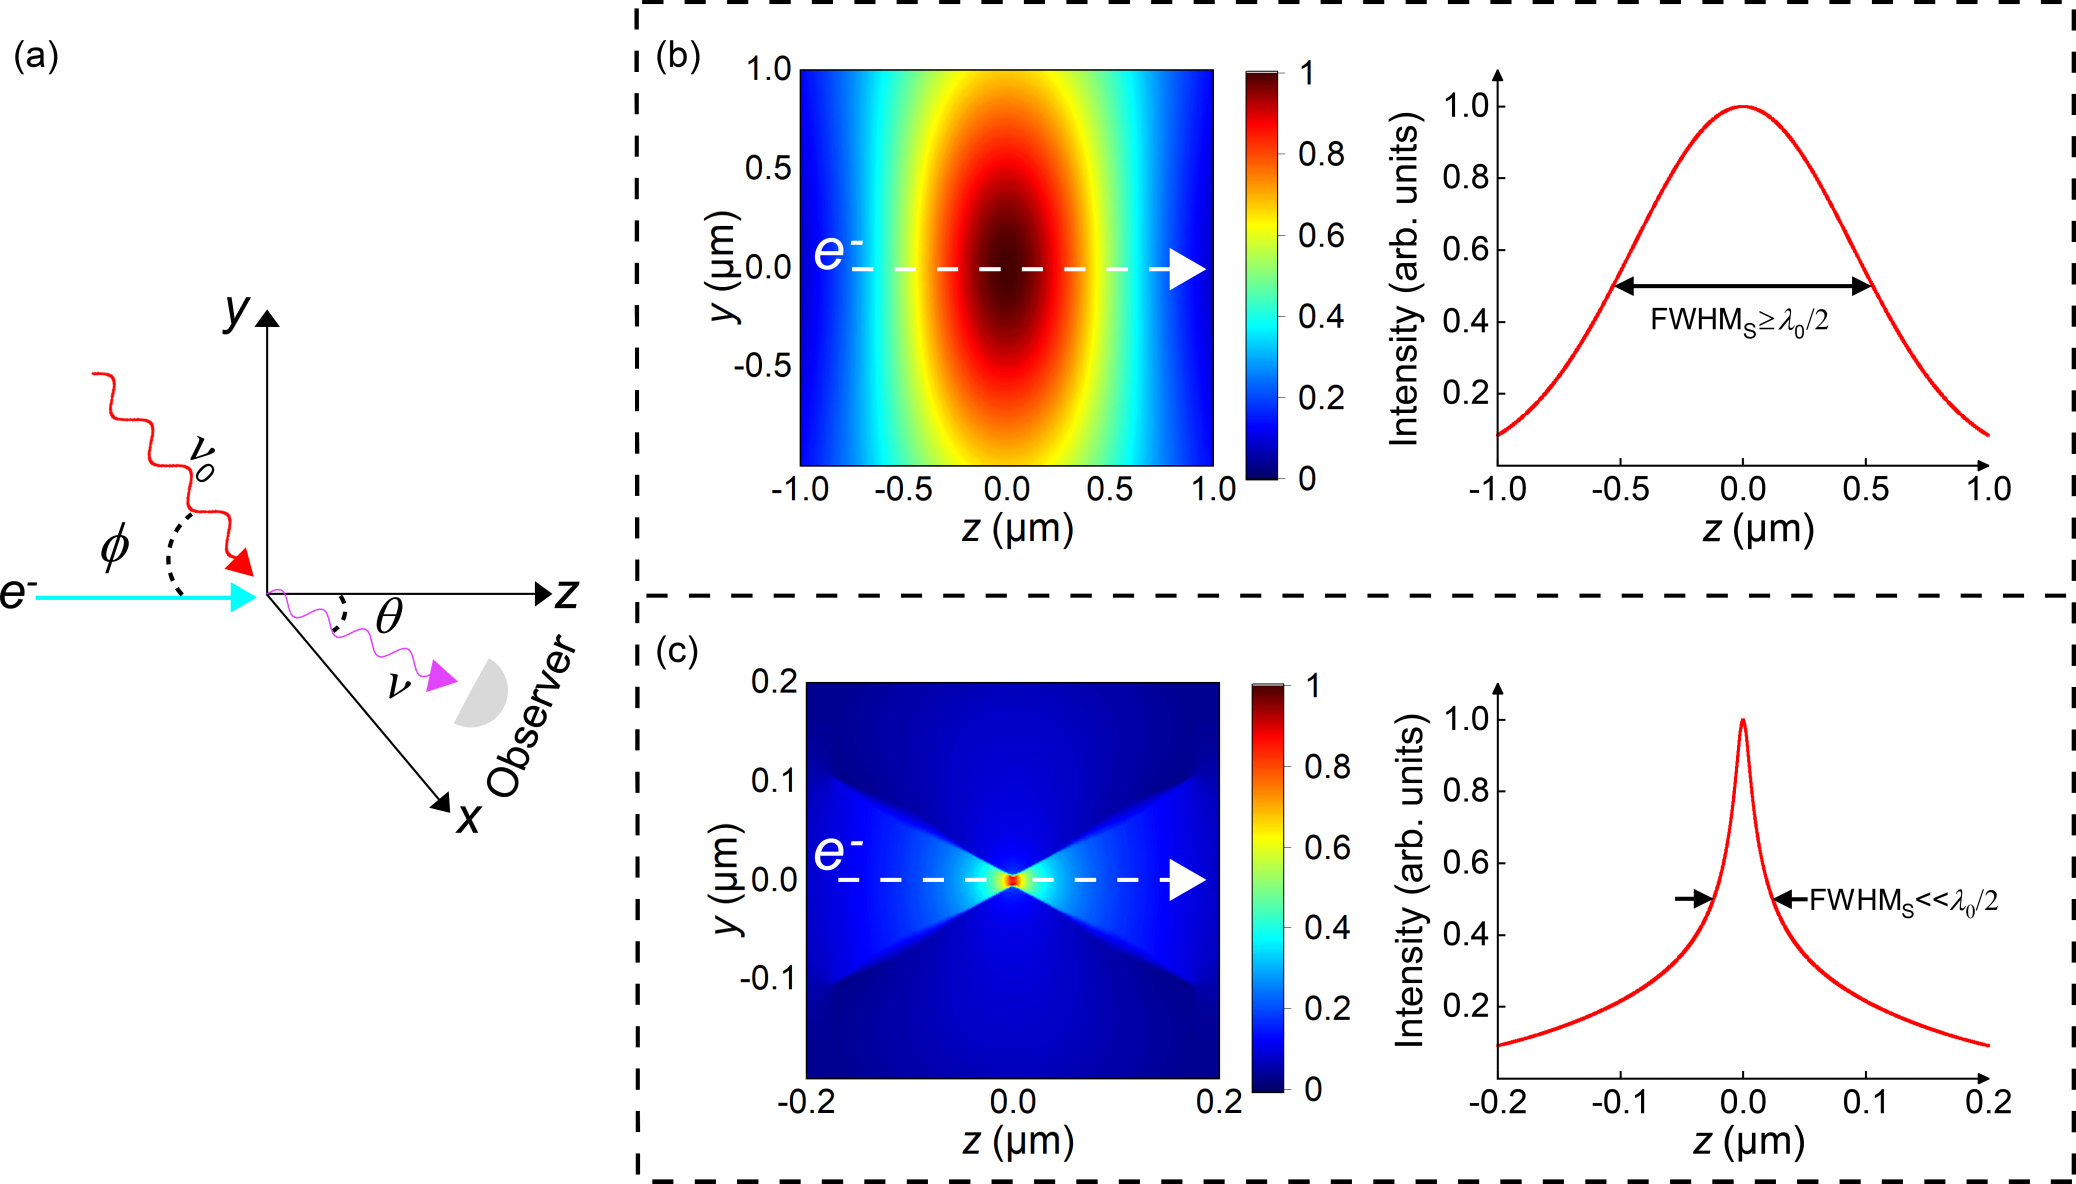
\includegraphics[width=0.85\linewidth]{pra_published_p2_img1.jpeg}
    \caption{\label{fig:scheme}打破光学脉冲半周期极限的原理示意图。（a）ICS 散射几何：相对论电子与约束光场中的光子碰撞，散射辐射以角度 $\theta$ 出射；（b）ICS 前辐射强度分布，$\text{FWHM} \approx \lambda/2$（受限于半周期极限）；（c）ICS 后辐射强度分布，$\text{FWHM} \ll \lambda/2$（打破半周期极限）。引自 Dang et al., Phys.\ Rev.\ A \textbf{112}, 013510 (2025)。}
\end{figure}

在典型参数下，该方案可以产生远小于半个光学周期的脉冲。以 0.4 THz 约束太赫兹场为例：3 MeV/1 fs 电子束散射后产生中心频率 26 THz（中红外）、脉宽 3.6 fs 的脉冲，仅对应 0.095 个光学周期；将电子能量提高至 15 MeV、脉宽压缩至 50 as 后，输出脉冲中心频率升至 0.49 PHz（可见光）、脉宽约 180 as，对应 0.091 个光学周期。图~\ref{fig:single-electron} 展示了单电子散射情形下的脉冲波形和频谱特征。

\begin{figure}[H]
    \centering
    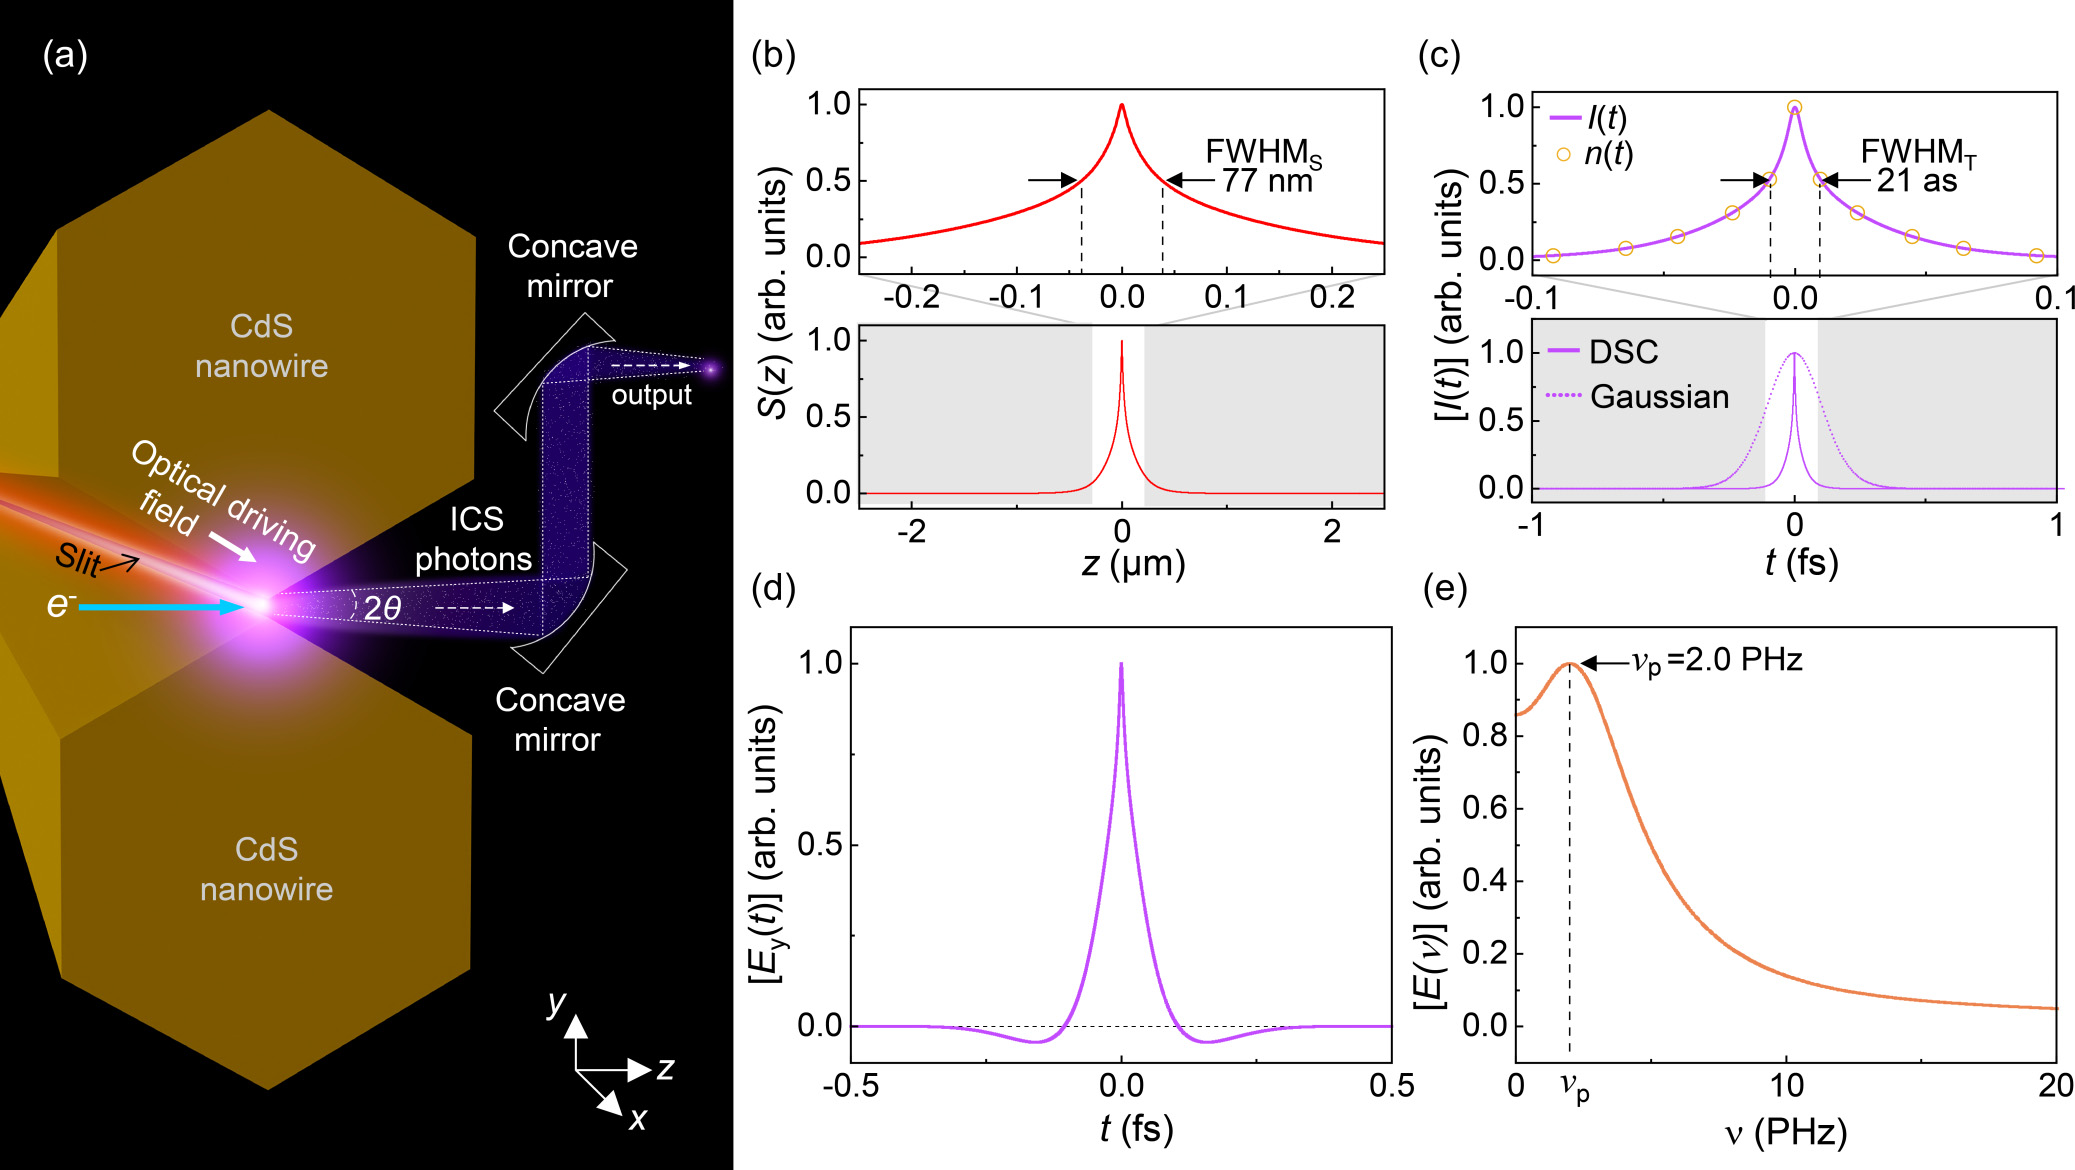
\includegraphics[width=0.85\linewidth]{pra_published_p3_img1.jpeg}
    \caption{\label{fig:single-electron}单电子逆康普顿散射产生深亚周期脉冲。（a）ICS 系统示意：CdS 纳米线间隙产生深亚波长约束光场，单电子垂直入射与光子碰撞；（b）约束光场空间强度分布 $S(z)$，$\text{FWHM}_S = 77$ nm；（c）散射脉冲时域波形（DSC vs.\ 高斯），$\text{FWHM}_T = 21$ as；（d）电场 $|E(t)|^2$ 时域分布；（e）频谱 $|E(\nu)|^2$，峰值频率 $\nu_p = 2.0$ PHz。引自 Dang et al., Phys.\ Rev.\ A \textbf{112}, 013510 (2025)。}
\end{figure}

进一步的分析表明，输出脉冲具有显著的单极振荡特征——与传统锁模或高次谐波方法产生的双极脉冲不同，本文方案的脉冲在时间轴上主要呈单向偏转。这一特性源于约束光场在电子静止系中的等效单周期结构经 Doppler 压缩后的不对称性。单极脉冲的载波-包络相位（Carrier-Envelope Phase, CEP）对波形极为敏感，为 CEP 物理研究提供了新的实验平台。

当电子束能量从 1 MeV 增加到 50 MeV 时，输出脉冲中心频率从太赫兹（约 1 THz）连续调谐至极紫外（约 30 PHz），脉宽从亚皮秒缩短至数十阿秒。约束光场的频率和空间尺度也独立影响输出参数——减小约束尺度可进一步缩短脉宽，但同时降低散射截面。图~\ref{fig:bunch} 展示了电子束团入射时的参数扫描结果。

\begin{figure}[H]
    \centering
    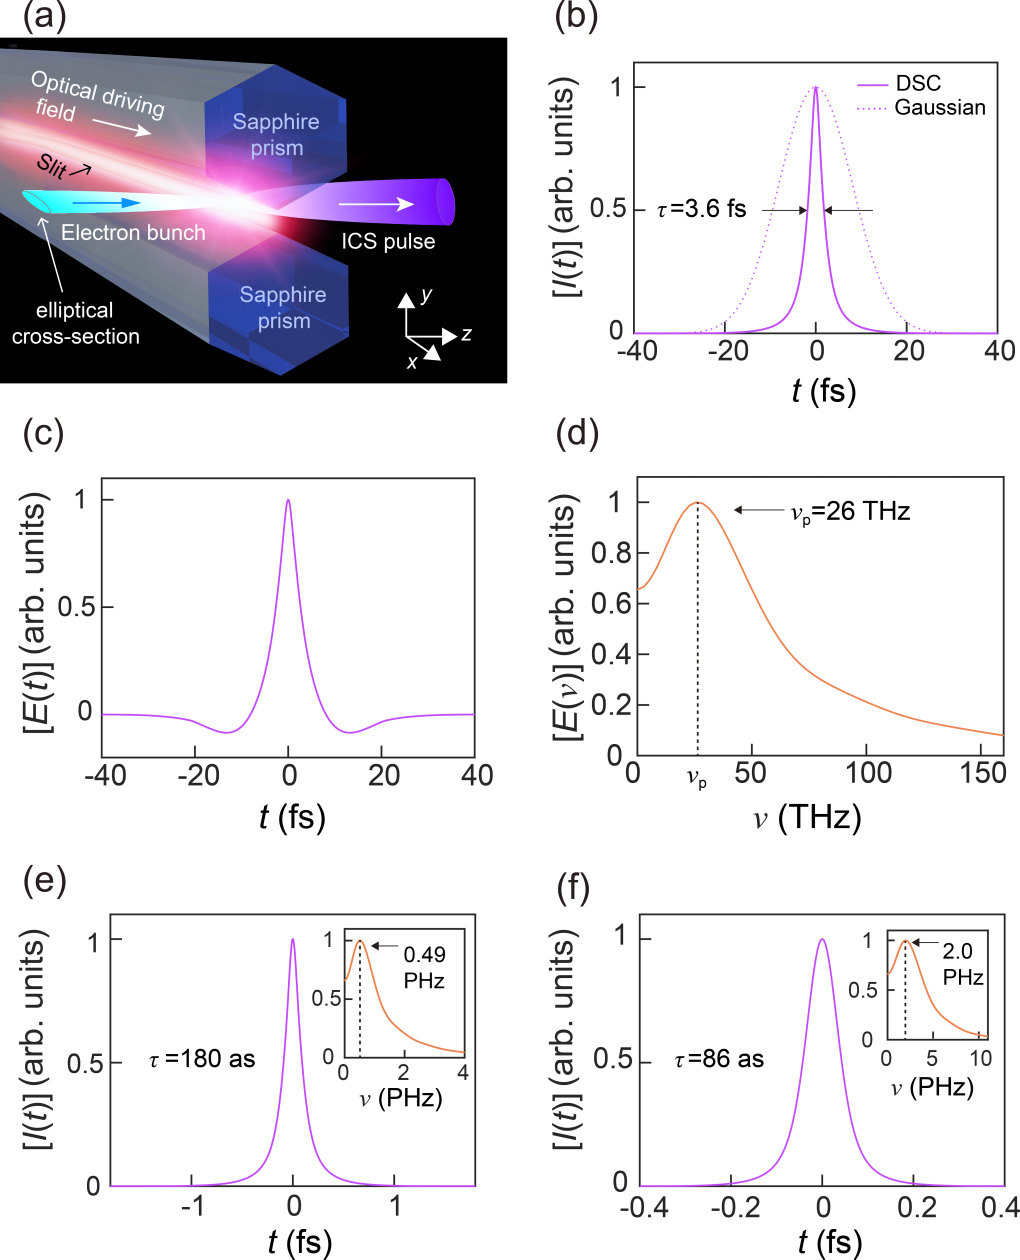
\includegraphics[width=0.85\linewidth]{pra_published_p5_img2.jpeg}
    \caption{\label{fig:bunch}电子束团入射时深亚周期脉冲的产生与压缩。（a）束团 ICS 系统示意：电子束团穿过蓝宝石棱镜耦合线对的约束光场；（b）输出脉冲时域波形（DSC vs.\ 高斯），$\tau = 3.6$ fs；（c）电场 $E(t)$；（d）频谱 $|E(\nu)|$，$\nu_p = 26$ THz（中红外）；（e）进一步提高电子能量后的压缩脉冲，$\tau = 180$ as，$\nu_p = 0.49$ PHz（可见光）；（f）极致压缩脉冲，$\tau = 86$ as，$\nu_p = 2.0$ PHz（极紫外）。引自 Dang et al., Phys.\ Rev.\ A \textbf{112}, 013510 (2025)。}
\end{figure}

本节工作已发表于 \textit{Physical Review A}（Hongliang Dang*, Jiaxin Gao*, Hao Wu, Yudong Zhang, Xin Guo, Limin Tong, Phys.\ Rev.\ A \textbf{112}, 013510, 2025）。

%------------------------------------------------------------------------------
\subsection{1.2 纳米线瓦量级连续波导波实验（已投稿）}
%------------------------------------------------------------------------------

1.1 节的理论方案需要纳米结构支持的高功率深亚波长约束光场。半导体纳米线是一维纳米光波导的理想载体，但在本工作之前，文献报道的半导体纳米线连续波（Continuous Wave, CW）导波功率仅限于毫瓦量级——与逆康普顿散射所需的场强差了四个数量级。提升导波功率成为实验推进的首要瓶颈。

本文采用化学气相沉积（CVD）法制备了高质量的 CdS 和 ZnO 单晶纳米线，并通过 SEM/TEM 表征确认了其晶体完整性和几何均匀性（图~\ref{fig:nanowire-sem}）。在此基础上构筑了"光纤—微纳光纤锥—纳米线"的级联耦合结构，实现了高效的光耦合输入与输出。

\begin{figure}[H]
    \centering
    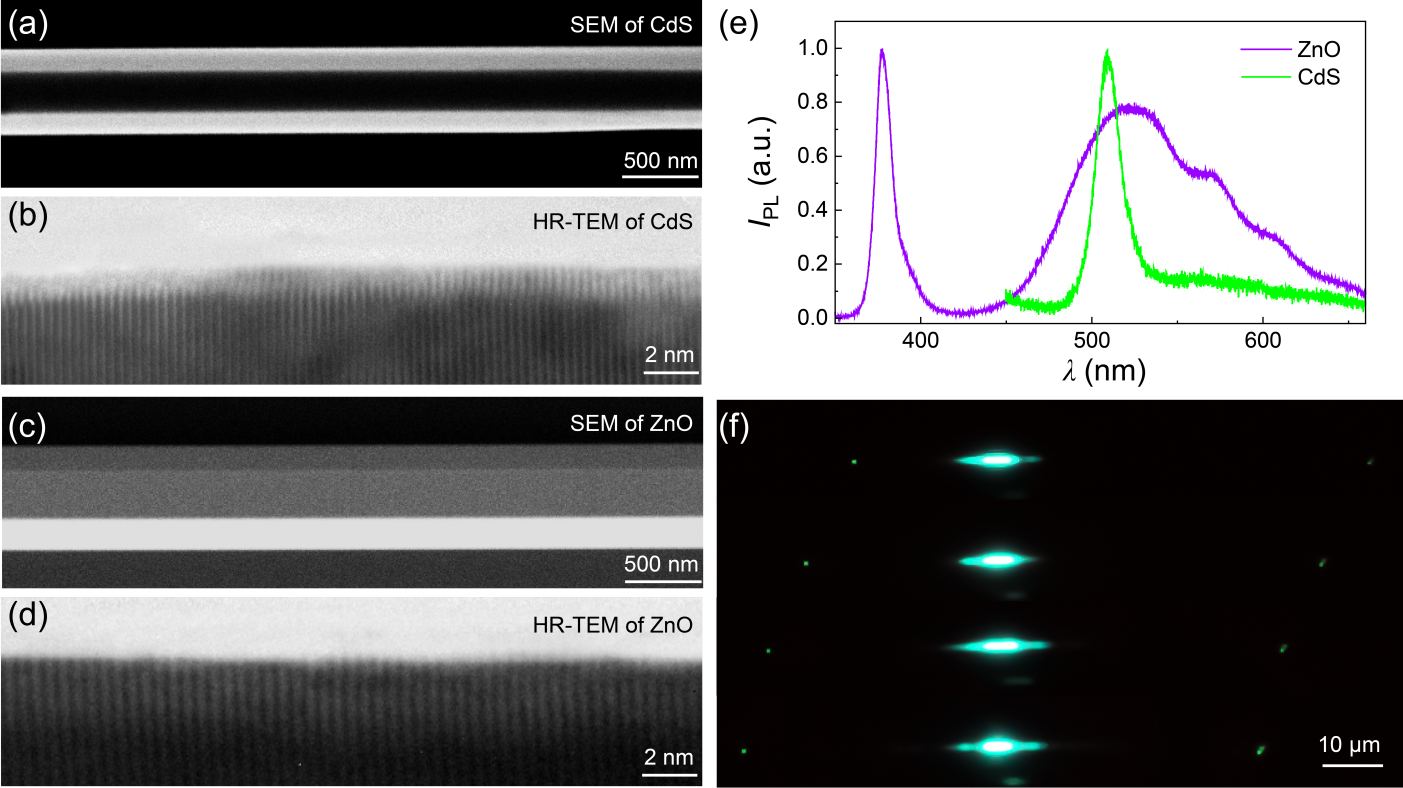
\includegraphics[width=0.85\linewidth]{apr_nanowire_p7_img1.png}
    \caption{\label{fig:nanowire-sem}CdS 和 ZnO 纳米线的结构与光学表征。（a）550 nm 直径 CdS 纳米线 SEM 图像；（b）130 nm 直径 CdS 纳米线 HR-TEM 图像（晶格条纹）；（c）690 nm 直径 ZnO 纳米线 SEM 图像；（d）480 nm 直径 ZnO 纳米线 HR-TEM 图像；（e）光致发光（PL）光谱：ZnO（紫色）与 CdS（绿色）；（f）纳米线导波光的光学照片。引自投稿论文 Dang et al.。}
\end{figure}

实验测得，直径 550 nm 的 CdS 纳米线在 1550 nm 波段的 CW 安全导波功率达到 2.5 W，对应功率密度约 $1.1 \times 10^{13}$ W/m$^2$——比先前文献纪录提高了约四个数量级。直径 690 nm 的 ZnO 纳米线在 1550 nm 导波 292 mW，在 532 nm 导波 33 mW。图~\ref{fig:high-power} 展示了导波功率随输入功率的变化曲线。

\begin{figure}[H]
    \centering
    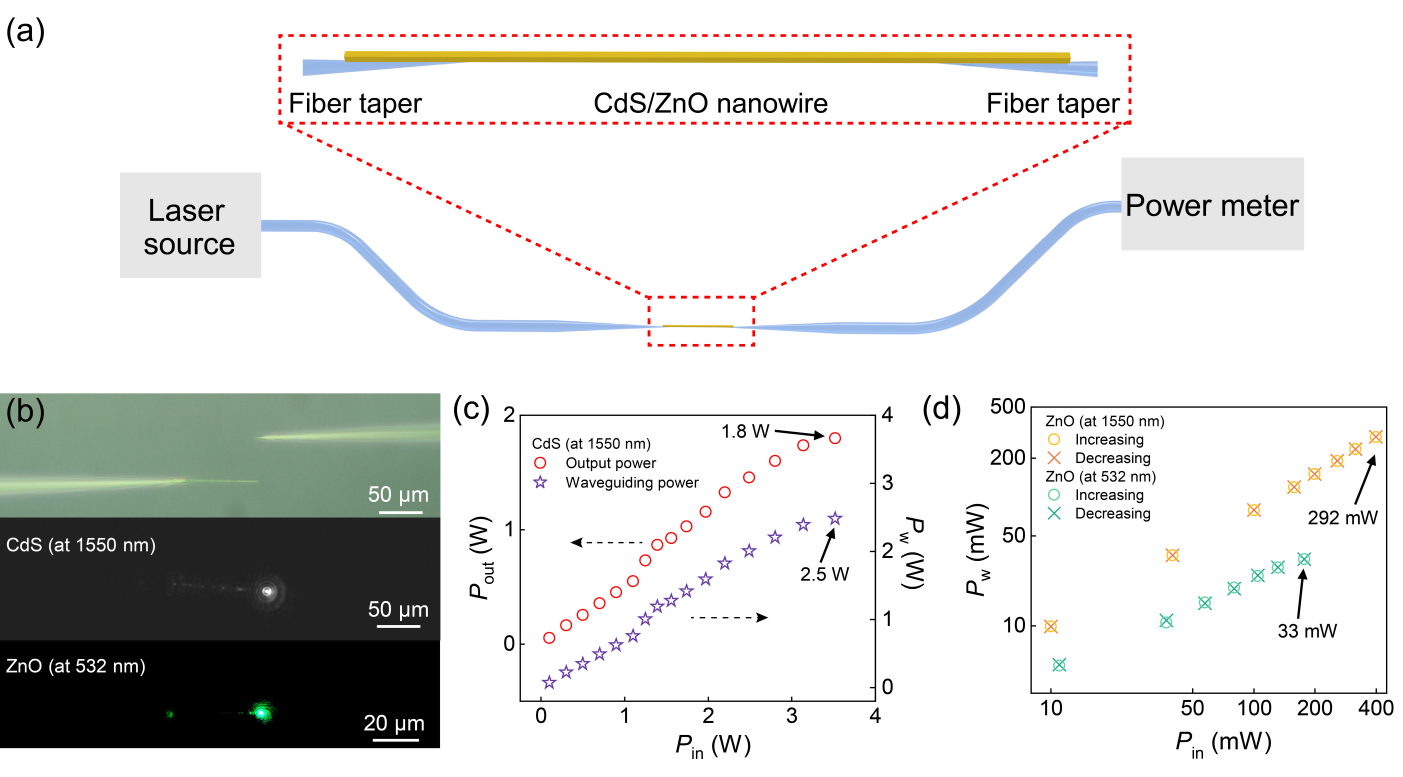
\includegraphics[width=0.85\linewidth]{apr_nanowire_p9_img1.png}
    \caption{\label{fig:high-power}纳米线高功率 CW 导波实验。（a）实验装置示意：EDFA 光源—光纤锥—纳米线—光纤锥—功率计；（b）CdS 纳米线（1550 nm，上）和 ZnO 纳米线（532 nm，下）的明场/暗场光学照片；（c）CdS 纳米线在 1550 nm 的输出—输入功率曲线，最大输出达 2.5 W；（d）ZnO 纳米线在 1550 nm（292 mW）和 532 nm（33 mW）的导波功率曲线。引自投稿论文 Dang et al.。}
\end{figure}

瓦量级导波得以实现，主要归因于两个因素：CVD 生长的单晶 CdS 在 1550 nm 波段带隙远离共振区，本征吸收损耗极低；级联耦合结构将耦合效率提升至实用水平。通过红外热成像实时监测纳米线温度，发现热点集中在耦合区域而非纳米线中段，说明耦合损耗（而非体吸收）是限制功率的主要因素。图~\ref{fig:harmonic} 展示了在高功率 CW 条件下观测到的谐波转换现象。

\begin{figure}[H]
    \centering
    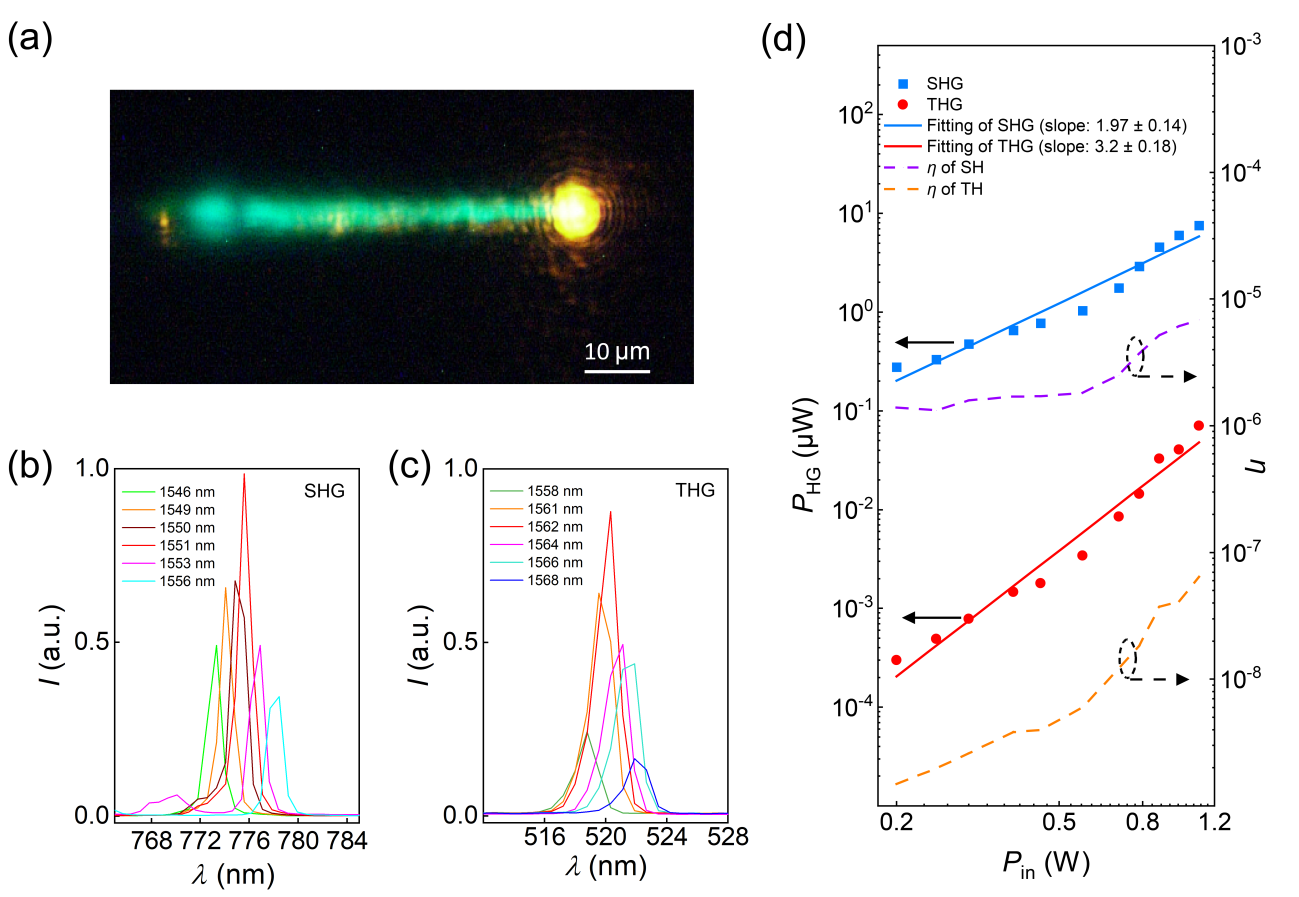
\includegraphics[width=0.85\linewidth]{apr_nanowire_p12_img1.png}
    \caption{\label{fig:harmonic}高功率 CW 导波下的非线性频率转换。SHG 转换效率达 $6.9 \times 10^{-6}$，与脉冲激发条件可比。引自投稿论文 Dang et al.。}
\end{figure}

本节工作已投稿至 \textit{Advanced Photonics Research}（Hongliang Dang, Zhanke Zhou, Jianbin Zhang, Liu Yang, Xin Guo*, Limin Tong*，初审提交，2026年5月）。

%------------------------------------------------------------------------------
\subsection{1.3 深亚波长约束光场逆康普顿散射的量子理论框架}
%------------------------------------------------------------------------------

1.1 节的处理采用了半经典近似——电子量子化、光场经典化。但当光场被约束到深亚波长尺度时，倏逝模的贡献不可忽略，虚动量光子对散射过程的修正可能使半经典结果产生系统性偏差。为此，本文从量子电动力学（QED）第一性原理出发，建立了适用于深亚波长约束光场的全量子散射理论。

具体做法是：对约束光场进行模展开，将传播模（$k_\perp < k_0$）与倏逝模（$k_\perp > k_0$）严格分离，对每类模式建立独立的产生-湮灭算符，再利用费米黄金定则计算包含近场修正的微分散射截面。主要结果包括：

\begin{itemize}
    \item \textbf{等效定理}：深亚波长约束光场的康普顿散射截面等价于不同平面波分量（含虚动量分量）标准散射截面的概率叠加——将复杂的近场散射简化为已知结果的加权求和。
    \item \textbf{虚光子效应}：高频虚光子传递更大的反冲能量，缩短有效作用时间，导致散射概率出现负偏离。在紧约束结构中这一效应尤为突出。
    \item \textbf{金属小孔模型}：紧邻小孔处实光子比例仅约 $3.2 \times 10^{-6}$，光场以虚光子为主导，半经典近似在该区域严重失效。
    \item \textbf{蓝宝石间隙结构}：间隙宽度减小 → 散射截面降低，但高频辐射分量增长。这一行为的物理根源是海森堡不确定性原理——空间局域化导致动量域展宽。
\end{itemize}

论文主体和补充材料正在撰写中。补充材料包含了从传播子推导到跃迁速率的完整六步推导链。

%------------------------------------------------------------------------------
\subsection{1.4 小孔极端约束光场的量子化}
%------------------------------------------------------------------------------

1.3 节的量子散射理论需要以约束光场的量子化描述为基础。对于小孔衍射——最典型的亚波长约束场景——Bethe（1944）的经典理论仅给出了远场衍射截面的偶极近似结果，尚未有完整的 QED 描述。本文填补了这一空白。

以理想导体薄屏上的亚波长圆孔（半径 $a \ll \lambda$）为模型，本文基于电偶极子—磁偶极子等效模型，发展了两套互补的量子化方案：

\begin{itemize}
    \item \textbf{库仑规范量子化}：通过三维模展开和 Weyl 角谱展开，推导出传播模和倏逝模统一适用的量子化磁矢势算符。关键技术是将三维波矢积分通过雅可比映射约化为二维角谱积分，解决了倏逝模 $k_z = i\kappa$ 时的归一化问题。
    \item \textbf{洛伦兹规范量子化}：引入 Gupta-Bleuler 条件处理非物理态，证明了倏逝模下标量光子和纵向光子仍精确抵消——这是对倏逝场量子化协变处理的重要验证。
    \item \textbf{经典极限验证}：在相干态期望值下，量子化场算符退化为经典表达式，远场辐射功率积分严格回归 Bethe 小孔衍射截面：
    \begin{equation}
        \sigma_{\text{Bethe}} = \frac{64}{27\pi} k_0^4 a^6
    \end{equation}
    \item \textbf{有限圆孔修正}：引入基于 Bessel 函数的形状因子，体现非理想点孔的有限尺寸效应。
\end{itemize}

图~\ref{fig:hole} 展示了小孔量子化模型的基本几何和场分布。

\begin{figure}[H]
    \centering
    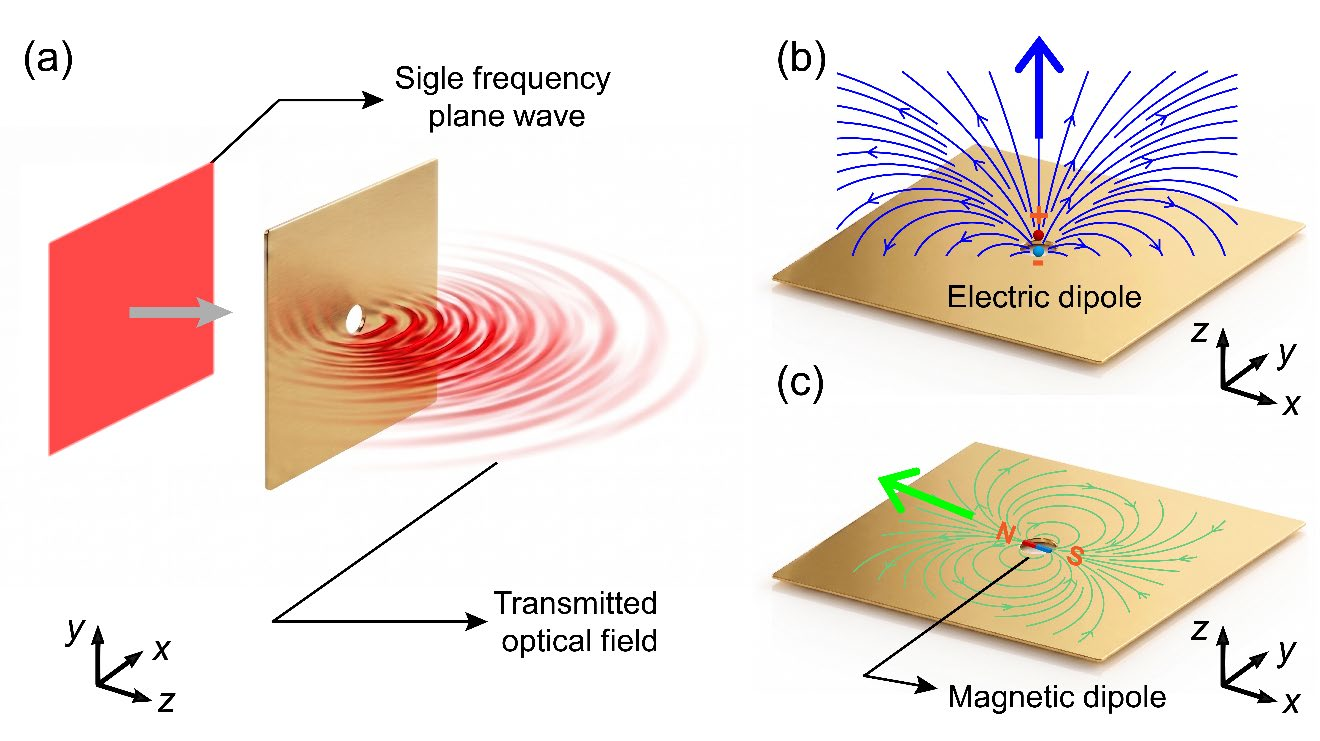
\includegraphics[width=0.7\linewidth]{hole_quantization_p3_img1.jpeg}
    \caption{\label{fig:hole}亚波长圆孔衍射的偶极等效模型。（a）单频平面波入射至理想导体薄屏上的亚波长圆孔（$a \ll \lambda$），透射场的衍射分布；（b）等效电偶极子辐射：沿 $z$ 轴的电偶极矩产生远场辐射；（c）等效磁偶极子辐射：沿 $x$ 轴的磁偶极矩。}
\end{figure}

论文主体和七节补充材料正在撰写中。

%------------------------------------------------------------------------------
\subsection{1.5 强场太赫兹源实验平台搭建}
%------------------------------------------------------------------------------

理论工作（1.1—1.4 节）为实验验证指明了方向。深亚周期脉冲的产生需要两个条件：强场深亚波长约束太赫兹驱动光场和高能电子束。其中太赫兹源是当前可最先推进的环节。

本文已完成强场太赫兹产生探测系统的可行性论证和设备审批。拟购置的系统基于铌酸锂（LiNbO$_3$）倾斜波前技术，主要技术指标如表~\ref{tab:thz-spec} 所示。

\begin{table}[H]
    \caption{\label{tab:thz-spec}强场太赫兹源系统主要技术指标}
    \begin{tabularx}{\linewidth}{c|X}
        \hline
        \textbf{参数} & \textbf{指标} \\
        \hline
        太赫兹单脉冲能量 & $\geq 2\;\mu\text{J}$ \\
        \hline
        中心频率 & 0.3—0.6 THz \\
        \hline
        最大平均功率 & $\geq 40\;\text{mW}$ \\
        \hline
        偏振态 & 竖直偏振 \\
        \hline
        探测方式 & 自由空间电光采样 \\
        \hline
        探测频谱范围 & 0.1—1.6 THz \\
        \hline
    \end{tabularx}
\end{table}

该系统依托北京航空航天大学吴晓君团队的铌酸锂倾斜波前和自由空间电光采样技术，计划一年内完成搭建与联合调试。系统中心频率（0.3—0.6 THz）与理论方案中的 0.4 THz 驱动场参数匹配，单脉冲能量 $\geq 2\;\mu\text{J}$ 可满足逆康普顿散射对场强的要求。配套的离轴抛物面反射镜将太赫兹脉冲聚焦至亚波长尺度，配合蓝宝石耦合线对结构即可产生深亚波长约束太赫兹光场。

%--------------------------------------------------------------------------
\section{二、尚须完成的任务}
%--------------------------------------------------------------------------

对照开题报告的研究计划，本文进展与原定时间线基本一致。开题时规划的四个阶段中，阶段 (i) 纳米线导波测试已完成，阶段 (ii) 核心理论工作基本完成、正在定稿。后续需推进的工作如下。

\subsection{2.1 理论工作完善}

完成逆康普顿散射量子理论和光场量子化两篇论文的最终修订，包括金属小孔模型的数值计算细节、有限圆孔 Bessel 形状因子的数值验证，以及全量子框架对半经典参数的修正计算。评估虚光子效应对输出脉冲波形和频谱的定量影响，确保所有解析推导与经典极限的一致性。

\subsection{2.2 实验平台搭建}

完成强场太赫兹源系统的设备购置与联合调试，实现单脉冲能量 $\geq 2\;\mu\text{J}$、中心频率 0.3—0.6 THz 的太赫兹脉冲输出。利用自由空间电光采样进行时域波形和频谱的全面表征，确认输出参数符合理论设计。同步推进深亚波长约束结构（蓝宝石棱镜耦合线对）的设计、制备与近场扫描验证。

\subsection{2.3 关键验证实验}

在太赫兹源和约束结构就绪后，协调皮秒高能电子束平台资源，开展约束光场中逆康普顿散射的初步实验。测量散射辐射的时域波形和频谱分布，与理论预言进行定量比对。

\subsection{2.4 学位论文撰写}

整合全部理论和实验成果，完成博士学位论文。

%--------------------------------------------------------------------------
\section{三、存在的问题}
%--------------------------------------------------------------------------

\subsection{3.1 理论计算的复杂性}

逆康普顿散射量子理论涉及倏逝模的多重求和与积分。在处理金属小孔等复杂几何时，角谱展开的收敛速度受结构参数影响较大，虚光子效应对散射截面的修正量级和符号依赖关系尚需系统的参数扫描来厘清。

\subsection{3.2 实验平台的资源协调}

实验验证需要强场太赫兹源和皮秒高能电子束的联合使用。太赫兹源正在推进购置，但电子束平台的预约使用需与相关课题组协调，实验窗口有限。浙江大学校内暂无兼具太赫兹强场产生和高能电子束的集成平台，跨实验室协调增加了周期的不确定性。此外，太赫兹光场与电子束的时空对准精度要求极高——相互作用区域为微米至亚毫米尺度，时间同步需达皮秒量级。

\subsection{3.3 约束光场的近场表征}

太赫兹波段的深亚波长约束光场缺乏成熟的近场表征手段。传统 SNOM 在可见和红外波段已有成熟方案，但推广到太赫兹面临探测器灵敏度和空间分辨率的双重困难。理论计算中的约束尺度（数十微米量级）虽大于 SNOM 针尖尺寸，但太赫兹探测器的噪声等效功率（NEP）远高于可见光探测器，弱信号探测需要多次平均或锁定放大技术。缺乏独立的近场表征将影响约束光场参数与理论计算的定量比对。

\subsection{3.4 纳米线与太赫兹波段的适配}

目前已完成的纳米线导波实验主要在近红外（1550 nm）和可见（532 nm）波段。理论方案中深亚周期脉冲的产生需要太赫兹波段的深亚波长约束，而太赫兹波长（300—1000 $\mu$m）远大于纳米线直径（数百 nm），模式匹配效率低。实际采用的是蓝宝石棱镜耦合线对结构，纳米线实验的价值在于验证了半导体材料在高功率密度下的可靠性。

%--------------------------------------------------------------------------
\section{四、拟采取的办法}
%--------------------------------------------------------------------------

\subsection{4.1 针对理论计算复杂性的解决方案}

采用分层计算策略：先用半经典近似（1.1 节）获得全局参数空间概览，再在关键参数点切换至全量子计算（1.3 节）进行精确修正。对于角谱展开的收敛性问题，引入物理截断判据——当倏逝模阶数对应的衰减长度小于电子束横向尺寸时，该模式贡献可忽略。同时发展基于物理直觉的近似方法，将虚光子效应用修正因子形式纳入半经典框架，降低全量子计算频次。

\subsection{4.2 针对实验平台协调的解决方案}

分阶段推进：(i) 当前至第 12 个月，优先完成太赫兹源搭建和参数表征，同步开展约束结构的数值仿真和制备工艺探索；(ii) 第 12—18 个月，协调电子束资源开展初步实验。时空对准方面，利用太赫兹电光采样信号的时间特征作为同步标记，配合精密位移台实现空间对准。

\subsection{4.3 针对近场表征困难的解决方案}

采用间接验证策略：利用太赫兹时域光谱（THz-TDS）的远场测量数据，结合理论模型反推近场分布。测量蓝宝石间隙结构的透射和反射波形，与有限元仿真（COMSOL）预测比对，验证约束结构的有效性。同时探索太赫兹电光采样的空间分辨能力——扫描探测光斑位置获取太赫兹场的空间分布，虽分辨率受限于探测光波长（约 800 nm），但足以区分约束区域与自由空间的场强差异。

\subsection{4.4 针对太赫兹波段适配的解决方案}

理论方案中太赫兹深亚波长约束不依赖纳米线结构，而是采用蓝宝石棱镜耦合线对。该结构已在理论计算中证明了产生 0.4 THz 约束光场的可行性。正在推进的太赫兹源设备（1.5 节）正是为该方案定制的。纳米线实验（1.2 节）验证了半导体在高功率密度下的可靠性，为未来多波段集成方案提供数据支撑。

\subsection{4.5 时间安排}

\begin{table}[H]
    \caption{\label{tab:timeline}后续研究时间安排}
    \begin{tabularx}{\linewidth}{c|X|X}
        \hline
        \textbf{时间段} & \textbf{主要任务} & \textbf{预期目标} \\
        \hline
        2026年6—8月 & 逆康普顿量子理论和光场量子化论文定稿 & 两篇论文投稿 \\
        \hline
        2026年6—12月 & 太赫兹源系统搭建与调试 & 太赫兹脉冲输出 $\geq 2\;\mu\text{J}$ \\
        \hline
        2026年9月—2027年3月 & 深亚波长约束结构设计、制备与表征 & 验证约束效果 \\
        \hline
        2027年1—6月 & 约束光场与电子束相互作用实验 & 初步实验结果 \\
        \hline
        2027年6—9月 & 学位论文撰写与修改 & 提交博士学位论文 \\
        \hline
    \end{tabularx}
\end{table}

\end{document}
